%%%%%%%%%%%%%%%%%%%%%%%%
% Method | Chapter 3
%%%%%%%%%%%%%%%%%%%%%%%%
\chapter{Method}
\label{chp:method}

\section{Research questions}
RQ1. Can the use of generative AI help improve the user experience in a data-intensive web application compared to traditional user interface methods?
\begin{itemize}
    \item RQ1.1. To what extent can generative AI affect the usability of a UI?

    With this research question we aim to explore the understandability of the UI. We will measure understandability by accounting for pondering time, and users asking for clarifications.

    \item RQ1.2. What are the key challenges for users using generative AI for data visualization in web applications?

    \item RQ1.3: Can generative AI help to improve perceived efficiency and task completion when working with a data-intensive web application?

    With this research question, we aim to explore efficiency in terms of tasks completed per time but also the perceived efficiency. We will measure efficiency by accounting for time spent per task and total tasks completed. The perceived efficiency will be measured through qualitative data collected in the exit interview.
    
\end{itemize}

\section{Literature review}
Search strings used on Scopus in order to locate the most relevant studies for our research on the impact of generative AI on user interfaces in data-intensive web applications, we have designed a search strategy to be employed within Scopus. The following search strings were used:

\begin{itemize}
    \item TITLE-ABS-KEY ( ( "generative AI" OR "generative artificial intelligence" ) AND ( "user interface" OR accessibility OR usability ) ) AND ( LIMIT-TO ( PUBSTAGE , "final" ) ) AND ( LIMIT-TO ( SUBJAREA , "COMP" ) OR LIMIT-TO ( SUBJAREA , "ENGI" ) OR LIMIT-TO ( SUBJAREA , "SOCI" ) OR LIMIT-TO ( SUBJAREA , "DECI" ) OR LIMIT-TO ( SUBJAREA , "BUSI" ) OR LIMIT-TO ( SUBJAREA , "ENVI" ) ) AND ( LIMIT-TO ( LANGUAGE , "English" ) )

    \item TITLE-ABS-KEY ( ( "data-intensive" OR "data intensive" ) AND "Web application" AND ( "user interface" OR accessibility OR usability ) ) AND ( LIMIT-TO ( PUBSTAGE , "final" ) ) AND ( LIMIT-TO ( SUBJAREA , "COMP" ) OR LIMIT-TO ( SUBJAREA , "ENGI" ) OR LIMIT-TO ( SUBJAREA , "SOCI" ) OR LIMIT-TO ( SUBJAREA , "DECI" ) OR LIMIT-TO ( SUBJAREA , "BUSI" ) OR LIMIT-TO ( SUBJAREA , "ENVI" ) ) AND ( LIMIT-TO ( LANGUAGE , "English" ) )
\end{itemize}



\section{Data Collection}
In our study are we using a mix of different methods to collect data. These include a demographic survey, an experiment and an exit interview. We are gathering quantitative data through the demographic survey, where we get information about our participants and their experience level. To collect data about "user experience, productivity, efficiency" we are going to perform an experiment where our participants perform data analysis tasks on a data-intensive web application. Half of the participants will use a traditional graphical user interface(GUI) and the other half will have access the same GUI as well as a generative AI that has access to the same data.  Following the completion of the experiment, we will conduct an exit interview with the participants to gather qualitative insights. During this interview, we aim to explore various aspects, including the participants' perceived efficiency and their experience using the application, both with and without AI. We will also inquire about any obstacles they encountered and assess whether the application was intuitive to use. 

During the experiment, the participants are prompted to verbalize their thoughts by thinking aloud\cite{thinkingAloud}, this will help us get as much data as possible from the few participants we are able to perform the experiment with.

\subsection{Demographic Survey(Google Forms):}
The purpose of this survey is to gather information about our participants to understand their background and experience with technology, their occupation as well as age. We will also inform the participants what the experiment will entail, including information about how the experiment will work, that they will be recorded and how the collected data will be used.

\begin{itemize}
    \item Inform and Get Consent: We are going to clearly explain the purpose of the study, what participation involves, risks, benefits, and confidentiality of responses. We will also ensure that our participants understand their rights, including the ability at any time without penalty. Obtain written or digital consent.
    \item Age: To understand the age distribution of our participants.
    \item Experience: Gauge the overall experience level with technology, specifically web applications and AI tools.
    \item Experience in What: Understand the domains of their experience, e.g., software development, design, data analysis, etc.
    \item Occupation Information: Collect data on their current job roles to understand their professional background.
    \item Inform About the Observation: Detail what the observation will entail, including the tasks to be performed, the use of recording equipment (if any), and how the collected data will be used.
\end{itemize}

\subsection{Session preparation (On-site)}
To be done before each session/participant. We will setup the application, with or without the AI component depending on the treatment for that participant. Have the necessary programs running and making sure it looks the same for each participant. Tasks will be prepared and printed out so the participant can read at their own discretion if necessary.

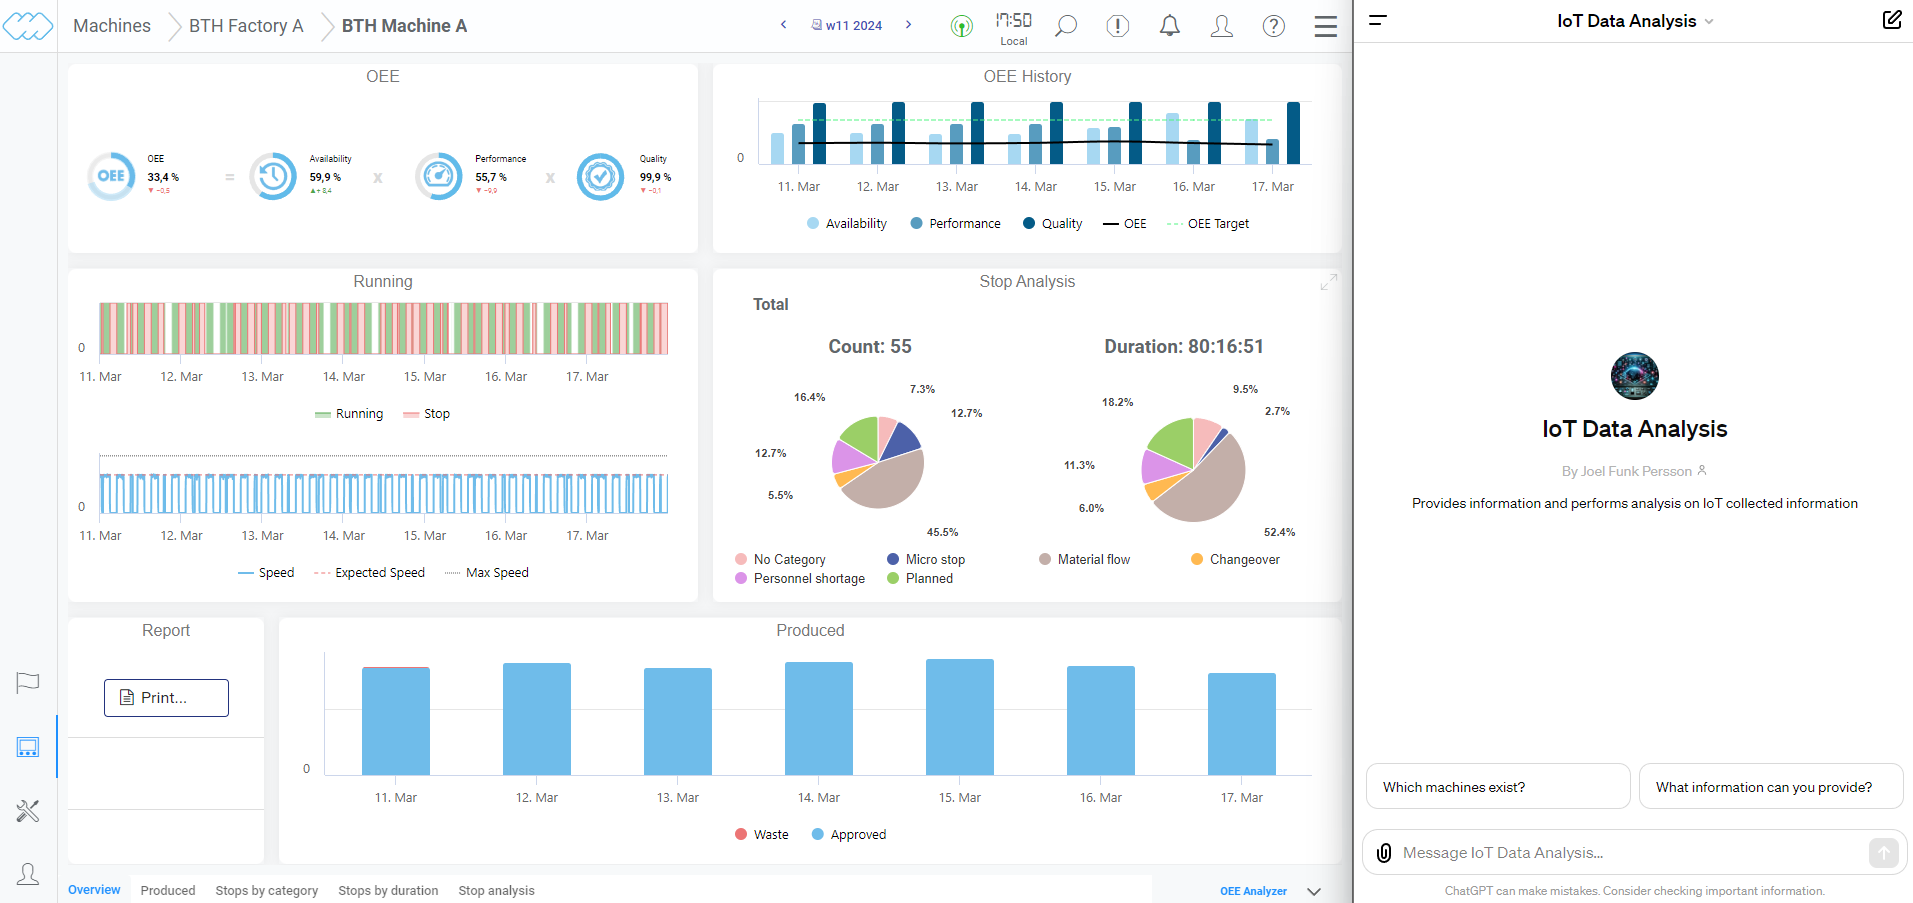
\includegraphics[width=\textwidth]{Images/experiment_ai_setup.png}

\begin{itemize}
    \item Setup Experiment Environment Beforehand: Ensure the application and all necessary tools are functioning and running correctly. Also that everything is set up exactly the same for each participant.
    \item Load Application: Have the application ready on the device that will be used for the observation.
    \item Load Generative AI Part: Ensure that the generative AI component of the application is set up and ready to interact with.
    \item Load Task Instructions: Prepare clear and concise instructions for the tasks participants will perform.
\end{itemize}

\subsection{Session steps (On-site) ~30 min}
To be performed with each participant. Th
\begin{itemize}
    \item Start Recording: Begin recording the session, ensuring to capture both the participant's interactions with the application and their verbal feedback.
    \item Explain the Application and Its Functionality: Provide a brief overview of the application, focusing on its purpose and key features.
    \item Explain Task Performance: We will describe how participants should perform the tasks by including any specific requirements/rules and guidelines. Explain that they will be given one task at a time, and upon completion or aborting of a task, the next one will be given to them. The tasks will start off short and easy and then increase in difficulty. Estimated time per task will vary, ranging from ~1-2 minutes to ~5-10.
    \item Instruct Them to Speak Out Loud: We will encourage participants to verbalize their thoughts, feelings, and frustrations as they interact with the application.
    \item Task Performance: Allow participants to start performing the tasks, observing and taking notes on their interactions and feedback. When a participant is done with a task, the next one will be given to them.
    \item Prompt to Speak if Necessary: If participants become silent, we will remind them to share their thoughts.
    \item Measure Task Completion Time: Record the time it takes for participants to complete each task.
    \item End of Observation: Conclude the task performance phase and stop the recording.
\end{itemize}

\subsection{Exit Interview (Semi-structured, On-site) ~15 min:}
\begin{itemize}
    \item Productivity Feelings: Ask participants about their perceived productivity while using the application. There we are focusing on their feelings rather than trying to quantify actual productivity.
    \item Ease of Use: Ask about the application's usability, how easy it was to accomplish basic tasks, how many mistakes (errors) were made, and whether participants found it intuitive and straightforward to navigate.
    \item Understanding and Starting Points: Assess whether participants knew how to start interacting with the application and the AI components, and if the UI effectively guided them in understanding what to do next.
    \item Satisfaction: Gather feedback on how satisfying participants found the application to use, including any particular features or interactions that stood out.
    \item General feedback: Ask the participant for any additional remarks, comments, or preferences about their experience that could be useful for evaluating the UI.
\end{itemize}

\subsection{Session conclusion}

\section{Validity and reliability}

\begin{comment}
    
\subsubsection{Validity}

Validity ensures that your study accurately reflects the concepts it intends to measure and the questions it aims to answer. Address the following types of validity:

\begin{enumerate}
    \item Construct Validity: Verify that the theory behind your constructs (like usability or efficiency measures) is sound. Ensure that the tools or methods you use to measure these constructs actually assess what they're supposed to. For instance, if you're studying user satisfaction with a generative AI interface, your measurement tools (such as questionnaires or observation checklists) should effectively capture all aspects of user satisfaction as defined by your research.
    \item Internal Validity: Focus on establishing a causal relationship between the independent variable (the introduction of generative AI into the interface) and the dependent variables (measures of user interaction, efficiency, etc.). Control for confounding variables that might affect the results, such as prior experience with similar technologies or individual user differences. Techniques such as randomization, control groups, or counterbalancing can be employed to enhance internal validity.
    \item External Validity: Discuss how your findings can be generalized to other settings, other user interfaces, or other populations. This might involve detailing how the participants were selected and the settings in which the experiments were conducted to argue that results are applicable to real-world scenarios.
    \item Content Validity (if applicable): This is about ensuring that the measures used cover all aspects of the construct being studied. For example, if your study aims to evaluate the completeness of a generative AI system in understanding user queries, the content validity would be concerned with how comprehensively the system's responses cover expected user queries in a given context.
\end{enumerate}

\subsubsection{Reliability}

Reliability pertains to the consistency of your measurement methods and the reproducibility of your results. Address these aspects:

\begin{enumerate}
    \item Test-Retest Reliability: This involves measuring the stability of your results over time. By administering the same test or observation under the same conditions on two or more occasions, you can check for consistency in your findings.
    \item Inter-Rater Reliability: Important for ensuring that qualitative data (like coding of open-ended responses or observational data) are consistently interpreted by different raters. Describe how multiple observers are trained and how their interpretations are standardized.
    \item Instrument Reliability: Ensure that any tools or technology used for data collection provide consistent and stable measurements across different test conditions and over time. For example, if you're using software to track user interactions, it should reliably capture the required data in every session.
\end{enumerate}
 
\end{comment}